\documentclass{report}
\usepackage[utf8]{inputenc}

%----- Configuración del estilo del documento------%
\usepackage{epsfig,graphicx}
\usepackage[left=2.5cm,right=2.5cm,top=1.8cm,bottom=2.3cm, margin=1in]{geometry}
%------ Paquetes matematicos --------%
\usepackage{amsmath}
\usepackage{amssymb}
\usepackage{amsthm}
\usepackage{amsmath}
\usepackage{tabularx}
\usepackage{fancyhdr}
\usepackage{lastpage}
\usepackage{verbatim}
\usepackage[shortlabels]{enumitem}
\usepackage{venndiagram}
\usetikzlibrary{shapes.geometric}
\usepackage{cancel}
\usepackage{hyperref}
\usepackage[T1]{fontenc}
\usepackage[spanish,es-nodecimaldot,es-tabla]{babel}
\usepackage{csquotes}
\usepackage{graphicx}
\usepackage{tocloft}
\graphicspath{{./figs/}}
\usepackage{setspace}
\usepackage{xcolor}

% paquete para la tabla
\usepackage{array}

% paquete para la bibliografía
% \usepackage[backend=biber]{biblatex}
% \addbibresource{resources/referencias/referencias.bib}




\begin{document}
    % Portada
	\begin{titlepage}
	\thispagestyle{empty}
	\begin{minipage}[c][0.17\textheight][c]{0.25\textwidth}
		\begin{center}
			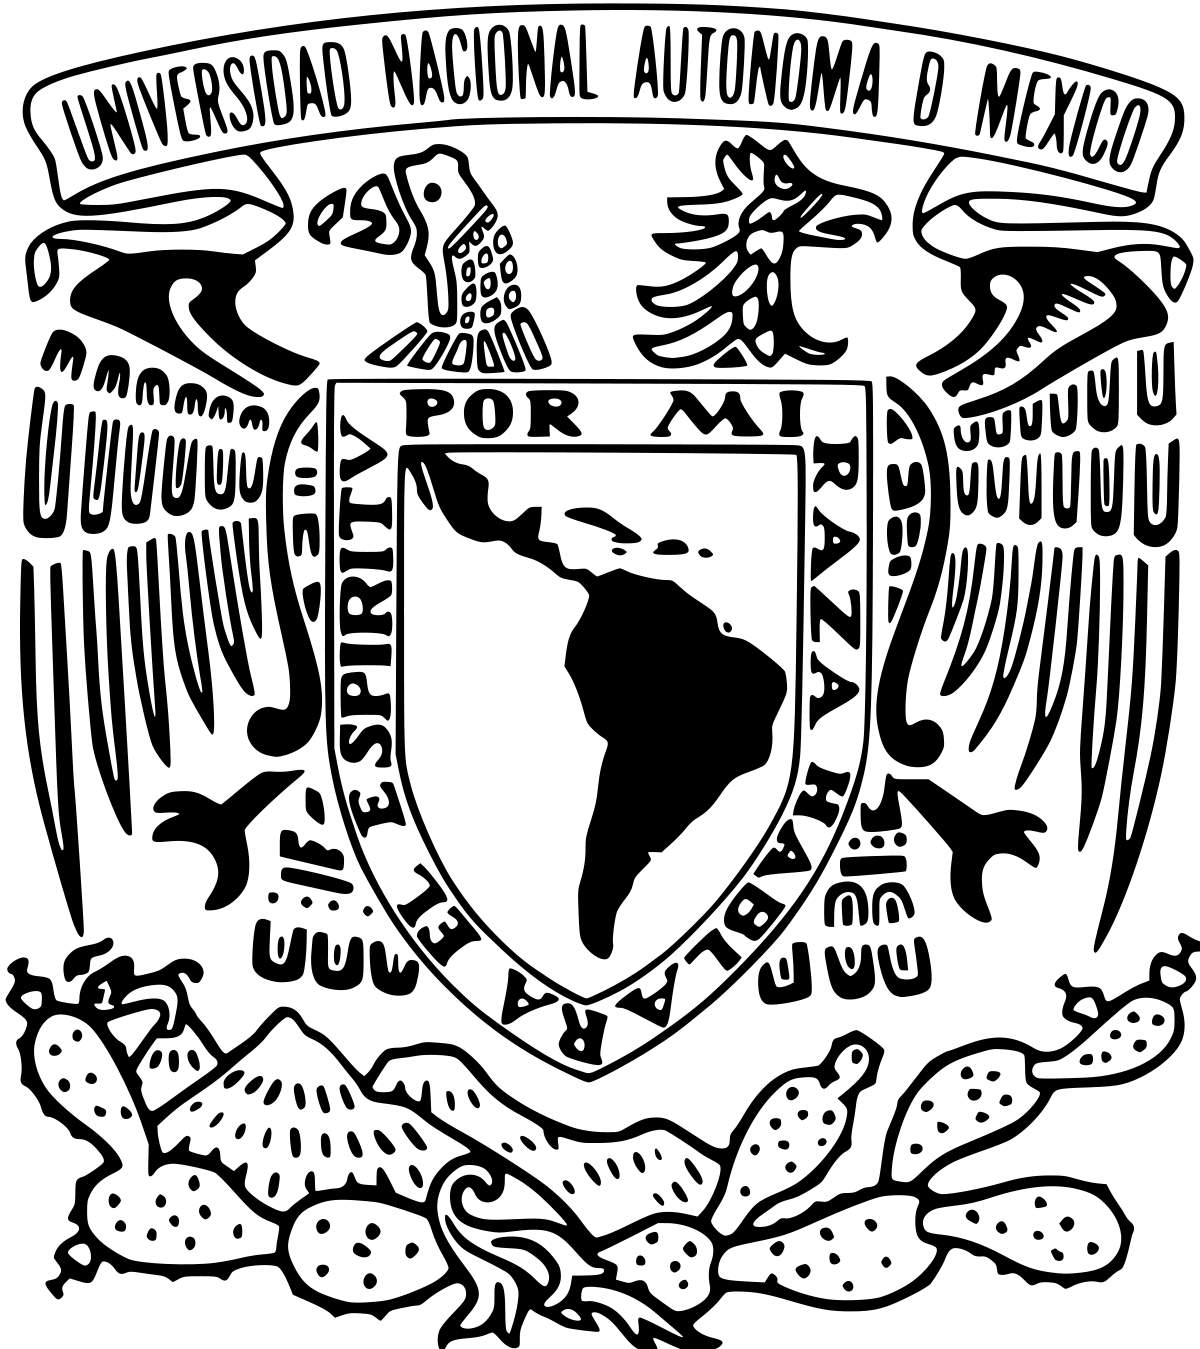
\includegraphics[width=3.5cm, height=3.5cm]{resources/Logo_UNAM.png}
		\end{center}
	\end{minipage}
	\begin{minipage}[c][0.195\textheight][t]{0.75\textwidth}
		\begin{center}
			\vspace{0.3cm}
			\textsc{\large Universidad Nacional Aut\'onoma de M\'exico}\\[0.5cm]
			\vspace{0.3cm}
			\hrule height2.5pt
			\vspace{.2cm}
			\hrule height1pt
			\vspace{.8cm}
			\textsc{Facultad de Ciencias}\\[0.5cm] %
		\end{center}
	\end{minipage}
	
	\begin{minipage}[c][0.81\textheight][t]{0.25\textwidth}
		\vspace*{5mm}
		\begin{center}
			\hskip2.0mm
			\vrule width1pt height13cm 
			\vspace{5mm}
			\hskip2pt
			\vrule width2.5pt height13cm
			\hskip2mm
			\vrule width1pt height13cm \\
			\vspace{5mm}
			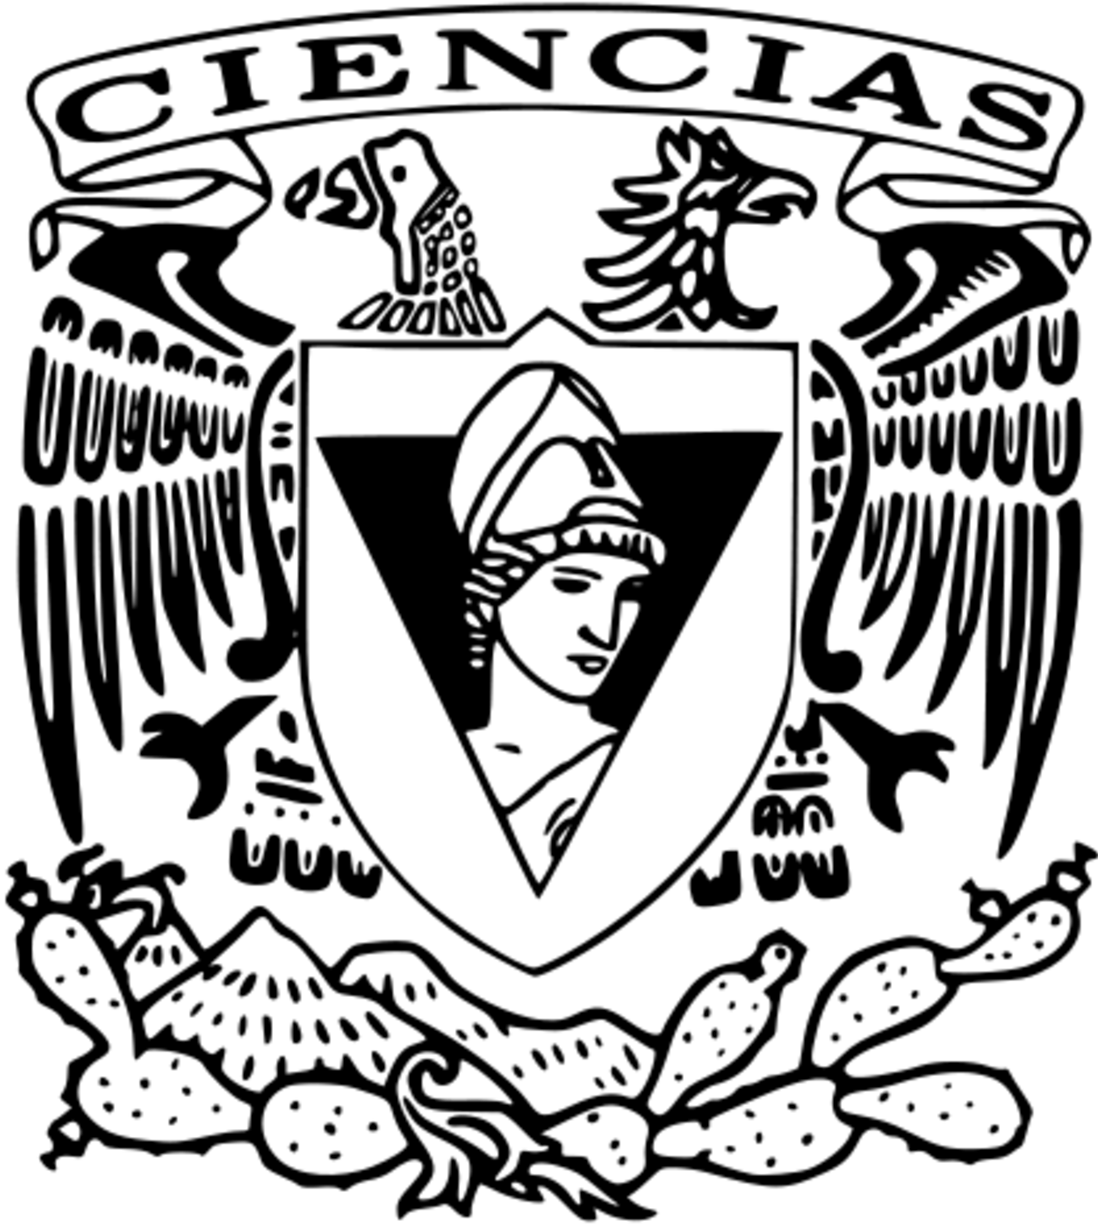
\includegraphics[height=4.0cm]{resources/Logo_FC.png}
		\end{center}
	\end{minipage}
	\begin{minipage}[c][0.81\textheight][t]{0.75\textwidth}
		\begin{center}
			\vspace{1cm}
			
			{\large\scshape Fundamentos de Bases de Datos - 7094}\\[.2in]
			
			\vspace{2cm}            
			
			\textsc{\LARGE \textbf{T}\hspace{1cm}\textbf{A}\hspace{1cm}\textbf{R}\hspace{1cm}\textbf{E}\hspace{1cm}\textbf{A}\hspace{1cm}\hspace{1cm}\textbf{4}}\\[2cm]
			\textsc{\Large{Equipo:}\normalsize \\
                \vspace{.3cm}
				\textbf{Del Monte Ortega Maryam Michelle - 320083527 \\
                \vspace{.2cm}
				\href{https://github.com/JuanSosaCiencias}{\textcolor{blue}{Sosa Romo Juan Mario - 320051926}} \\
                \vspace{.2cm}
				Castillo Hernández Antonio - 320017438 \\
                \vspace{.2cm}
                Erik Eduardo Gómez López - 320258211 \\
                \vspace{.2cm}
                Julio César Islas Espino - 320340594}}\\[0.5cm]     
			
			\textsc{{Fecha de entrega: \\ \textbf{10 de Octubre de 2024}}}\\[0.5cm]        
			
			\textsc{{Profesor: \\ \textbf{M. en I. Gerardo Avilés Rosas}}}\\[0.5cm]  
			
			\textsc{Ayudantes: \\ \textbf{Luis Enrique García Gómez \\ Kevin Jair Torres Valencia \\ Ricardo Badillo Macías \\ Rocío Aylin Huerta González
			} }
			
			
			\vspace{0.5cm}
		\end{center}
	\end{minipage}
\end{titlepage}


    % Titulo
	\begin{center}
		{\let\newpage\relax\chapter*{Tarea 5}}
	\end{center}

    % Preguntas  

    \begin{enumerate}%[label=\alph*.]
        \item \begin{center}
    \textbf{Menciona 5 diferencias sentre almacenar la informacion utilizando un sistema de archivos o almacenarla utilizando una BDD.}
\end{center}

\begin{enumerate}
    \item \textbf{Estructura de Datos:} Los sistemas de archivos son simples colecciones de archivos sin relación entre ellos, mientras que             las bases de datos organizan los datos de manera estructurada y con relaciones lógicas.
    \item \textbf{Redundancia:} La redundancia de datos es alta en los sistemas de archivos, ya que los mismos datos pueden aparecer en                 múltiples lugares. En las bases de datos, la redundancia se minimiza mediante normalización.
    \item \textbf{Consistencia de Datos:} Los sistemas de archivos tienen problemas de inconsistencia cuando los datos se modifican en                 varios archivos. En las bases de datos, las actualizaciones se reflejan de manera consistente en todas las instancias de los datos.
    \item \textbf{Seguridad:} Los sistemas de archivos suelen ofrecer menos seguridad, mientras que las bases de datos incluyen medidas de             seguridad avanzadas como control de acceso y encriptación. 
    \item \textbf{Copia de Seguridad y recuperación:} Los sistemas de archivos no cuentan con mecanismos automatizados de respaldo y                     recuperación, mientras que las bases de datos generalmente incluyen estas funciones para proteger la información.\\
\end{enumerate}
\cite{guru99, sooluciona}

\vspace{.5cm}



        
        \item \textbf{¿Qué ventajas y desventajas encuentras al trabajar con un Sistema de Bases de Datos
considerando que se planea implantar este sistema en una empresa de telemarketing?} \\

En primera instancia tenemos que reconocer que el telemarketing es una técnica publicitaria que es utilizada por las empresas para contactar con potenciales clientes y hablarles acerca de sus productos o servicios . \\

Hay muchas empresas a lo largo del mundo que hacen de esta estrategia su principal manera de operar, catalogándose en mayor o menor medida como empresas de telemarketing y si bien cada empresa decide como gestionar sus recursos para así poder llegar a su publico objetivo, el telemarketing cuenta con una serie de ventajas y desventajas enumeradas de la siguiente manera las cuales pueden hacer que una empresa se decante por este sistema o no: \\


\begin{table}[h!]
    \centering
    \begin{tabular}{|p{6cm}||p{6cm}|}
        \hline
        \textcolor{blue}{\textbf{Ventajas}} & \textcolor{Red}{\textbf{Desventajas}} \\ \hline 
        Se tiene un trato mas directo con los potenciales clientes & Si se utiliza de manera inadecuada puede afectar negativamente a la reputación de la empresa \\ \hline
        Permite entrar en contacto con un gran número de clientes en poco tiempo & En algunos países existen ciertas restricciones para esta clase de técnicas \\ \hline 
        Permite ofrecer una gran cantidad de información sobre el producto o servicio en cuestión  & Requiere una inversión en formar a los agentes y que estos sigan las buenas practicas de la empresa \\ \hline
        Se puede llamar a cualquier parte del mundo, lo cual asegura que nuestra empresa pueda darse a conocer en otras fronteras & La tasa de conversión es baja\\ \hline
    \end{tabular}
    \caption{Ventajas y desventajas de un Sistema de Telemarketing \cite{boada_cyberclick_2023}} 
\end{table}

Así mismo el telemarketing puede utilizarse de distintas maneras y estas varían de acuerdo a la campaña y objetivos de la empresa. Pero volviendo al punto principal de la pregunta, algunas de las posibles ventajas y desventajas de implemmentar un sistema de base de datos en alguna empresa de telemarketing podrian ser las siguientes:\\


\begin{table}[h!]
    \centering
    \begin{tabular}{|p{6cm}||p{6cm}|}
        \hline
        \textcolor{green}{\textbf{Ventajas}} & \textcolor{purple}{\textbf{Desventajas}} \\ \hline
        Organización y gestión eficiente de datos & Altos costos de implementación y mantenimiento continuo. \\ \hline
        Generación de análisis detallados e historial de datos. & Trabajo extra para integración con sistemas existentes y necesidad de capacitación del personal. \\ \hline
         Automatiza las tareas repetitivas y hay una reducción de errores manuales. & Riesgo de interrupciones por fallos del sistema y necesidad de ajustes por actualizaciones. \\ \hline
        Tiene la capacidad para manejar más datos y mas personalización según necesidades específicas. &  Riesgos de seguridad y necesidad de cumplir con normativas de privacidad. \\ \hline
        Existe un control de acceso a datos sensibles y así como también un respaldo de datos. & Existen riesgos por parte de entradas de datos incorrectos y problemas de duplicados. \\ \hline
    \end{tabular}
    \caption{Ventajas y desventajas de un Sistema de BD en una empresa de telemarketing}
    \cite{adSalsa_2024}
\end{table}

        
        \item \textbf{Investiga que cuáles son las Reglas de Codd y explica con tus propias palabras cada una de ellas. Indica por qué
consideras que son importantes.}\vspace{.3cm}

        
        \item \begin{center}
    \textbf{Para cada política que investigaron, ¿cuáles son sus ventajas y desventajas\end{center}
\begin{itemize}

    \item \textbf{CASCADE}:
    
    \textbf{Ventaja}: Facilita la gestión automática de datos relacionados, eliminando o actualizando los registros dependientes de manera automática, lo que reduce el trabajo manual y asegura la coherencia entre las tablas.
    
    \textbf{Desventaja}: Es peligrosa, ya que una eliminación en cascada podría borrar muchos registros relacionados de forma accidental, lo que podría resultar en la pérdida de diversos datos importantes.
    
    \vspace{0.5cm}
    
    \item \textbf{SET NULL}:
    
    \textbf{Ventaja}: Permite mantener los registros relacionados, pero indicando que la relación con la tabla principal ya no es válida, asignando un valor \texttt{NULL}. Es útil cuando se desea conservar los datos secundarios sin una relación activa.
    
    \textbf{Desventaja}: Puede generar inconsistencias si se permite que muchos campos se queden en \texttt{NULL}, lo que complica analizar los datos. Además, no es aplicable si la columna no permite valores \texttt{NULL}.
    
    \vspace{0.5cm}
    
    \item \textbf{SET DEFAULT}:
    
    \textbf{Ventaja}: Asigna un valor predeterminado en los registros relacionados cuando se elimina o actualiza un registro en la tabla principal, lo que puede ser útil para mantener datos válidos en los registros secundarios.
    
    \textbf{Desventaja}: Podría introducir datos incorrectos o inconsistentes si el valor predeterminado no refleja adecuadamentevlos datos. Esto podría generar confusión o errores en los reportes.
    
    \vspace{0.5cm}
    
    \item \textbf{RESTRICT}:
    
    \textbf{Ventaja}: Protege contra la eliminación o actualización accidental de registros importantes, asegurando que no se puedan eliminar registros si existen dependencias en otras tablas. Esto previene la creación de registros huérfanos.
    
    \textbf{Desventaja}: Puede ser demasiado restrictiva en algunos casos, bloqueando operaciones que podrían ser necesarias, lo que podría generar errores al intentar gestionar los datos.
    
    \vspace{0.5cm}
    
    \item \textbf{NO ACTION}:
    
    \textbf{Ventaja}: Similar a \texttt{RESTRICT}, impide la eliminación o actualización de registros relacionados, pero la validación ocurre al final de la transacción, lo que podría ser útil en transacciones complejas.
    
    \textbf{Desventaja}: Al validar la integridad referencial al final de la transacción, pueden generarse errores que sean difíciles de manejar, especialmente si ocurren al final de un proceso complejo.

    \vspace{0.5cm}
    
\end{itemize}

        
        \item \begin{center}
    \textbf{Con base a lo anterior, ¿cuál política utilizarán para su esquema, y porqué motivo?}
\end{center}

Para todas nuestras llaves foránea usamos la política on delete cascade y on update cascade.

Lo anterior debido a 

        
        \item Se tiene la siguiente relación:
\begin{center}
    \textbf{R(idEnfermo, idCirujano, fechaCirugía, nombreEnfermo, direcciónEnfermo, nombreCirujano, nombreCirugía, medicinaSuministrada, efectosSecundarios)}
\end{center}
\begin{itemize}
    \item \textbf{Expresa las siguientes restricciones en forma de dependencias funcionales:}
    
    \begin{itemize}
        \item A un enfermo sólo se le da una medicina después de la operación. 
        \item Si existen efectos secundarios estos dependen sólo de la medicina suministrada.
        \item Sólo puede existir un efecto secundario por medicamento.
    \end{itemize}

    Podemos satisfacer las restricciones con:
    \begin{itemize}
        \item $idEnfermo, fechaCirugia \rightarrow medicinaSuministrada$

        Esto porque indica que para un enfermo específico en una fecha de cirugía específica, solo se le puede administrar una medicina. Lo cuál cubre la primera restricción. 

        Ocupamos tanto el idEnfermo como la fecha de la cirugía, o de otra manera no sabríamos a que enfermo administrarle la medicina después de su cirugía (fecha).

        \item $medicinaSuministrada \rightarrow efectosSecundarios$

        Aquí cumplimos con las dos restricciones que faltaban, porque asignamos a cada medicina un único efecto secundario. En este caso, es una dependencia funcional simple ya que solo ocuparemos la medicina para saber qué efecto secundario tiene. 
    \end{itemize}
    
    \item \textbf{Especifica otras dependencias funcionales o multivaluadas que deban satisfacerse en la relación \textbf{R}. Por cada una que definas, deberá aparecer un enunciado en español como en el inciso anterior.}

    Otras dependencias funcionales en \textbf{R} son:
    \begin{itemize}[label=$\heartsuit$]
        \item Cada enfermo tiene un único nombre y una única dirección
        \[idEnfermo \rightarrow nombreEnfermo, direccionEnfermo\]
        \item Cada cirujano tiene un único nombre
        \[idCirujano \rightarrow nombreCirujano\]
        \item Una cirugía realizada por un cirujano a un enfermo sólo puede ocurrir en una fecha determinada
        \[idEnfermo, idCirujano, nombreCirugia \rightarrow fechaCirugia\]
        \item Un enfermo en una fecha específica solo puede tener una cirugía y esta debe ser realizada por un único cirujano
        \[idEnfermo, fechaCirugia \rightarrow nombreCirugia, idCirujano\]
        \item El enfermo y la fecha de cirugía determina el cirujano que realizó la operación
        \[idEnfermo, fechaCirugia \rightarrow idCirujano\]
        \item El cirujano y la fecha determina qué cirugía se está realizando en ese momento
        \[idCirujano, fechaCirugia \rightarrow nombreCirugia\]
       
        \item El nombre de la cirugía determina qué medicinas pueden ser suministradas después de la operación
        \[nombreCirugia \twoheadrightarrow  medicinaSuministrada\]
        Esta es una dependencia multivaluada ya que una cirugía puede tener varias medicinas posibles
        \item La combinación de enfermo, cirujano y fecha determina unívocamente todos los demás atributos de la relación

        \begin{center}
            
        $idEnfermo, idCirujano, fechaCirugia \rightarrow nombreEnfermo, direccionEnfermo, nombreCirujano, nombreCirugia,$
        
        $medicinaSuministrada, efectosSecundarios$
        \end{center}
        

    \end{itemize}
    Estas dependencias surgen de restricciones pensadas por nosotros mismos, por lo que podrían no ser generales en un contexto de un hospital real.
    
    \item \textbf{Normaliza utilizando el conjunto de dependencias establecido en los puntos anteriores.}

    Tenemos el siguiente conjunto de dependencias:

    \textbf{F} = \{
    
    1. idEnfermo $\rightarrow$ nombreEnfermo, direccionEnfermo
    
    2. idCirujano $\rightarrow$ nombreCirujano
    
    3. idEnfermo, idCirujano, nombreCirugia $\rightarrow$ fechaCirugia
    
    4. idEnfermo, fechaCirugia $\rightarrow$ nombreCirugia, idCirujano
    
    5. idEnfermo, fechaCirugia $\rightarrow$ idCirujano
    
    6. idCirujano, fechaCirugia $\rightarrow$ nombreCirugia
    
    7. nombreCirugia $\twoheadrightarrow$ medicinaSuministrada
    
    8. idEnfermo, idCirujano, fechaCirugia $\rightarrow$ nombreEnfermo, direccionEnfermo, nombreCirujano, nombreCirugia, medicinaSuministrada, efectosSecundarios
    
    9. idEnfermo, fechaCirugia $\rightarrow$ medicinaSuministrada
    10. medicinaSuministrada $\rightarrow$ efectosSecundarios
\}

Como tenemos una dependencia multivaluada, usaremos $4FN$

Debido a la DF 8, la llave candidata es:

\{idEnfermo, fechaCirugia\}+=
\{idEnfermo fechaCirugia, nombreEnfermo direccionEnfermo, nombreCirugia idCirujano, nombreCirujano, medicinaSuministrada, efectosSecundarios\}


\textbf{PASO 1:} Primera violación a 4FN
\begin{itemize}
    \item La DMV nombreCirugia $\twoheadrightarrow$ medicinaSuministrada es una violación ya que nombreCirugia no es superllave
    
    \item Dividimos en dos relaciones:
    \begin{itemize}[label=\textcolor{magenta}{$\bigstar$}]
        \item $R_1$(nombreCirugia, medicinaSuministrada) 
        
        Ya está en $4FN$ pues no tiene DMVs no triviales
        \item $R_2$(idEnfermo, idCirujano, fechaCirugia, nombreEnfermo, direccionEnfermo, nombreCirujano, nombreCirugia, efectosSecundarios) con:
        \begin{itemize}
            \item idEnfermo $\rightarrow$ nombreEnfermo, direccionEnfermo
            \item idCirujano $\rightarrow$ nombreCirujano
            
            \item idEnfermo, fechaCirugia $\rightarrow$ nombreCirugia, idCirujano
        \end{itemize}
    \end{itemize}
\end{itemize}


\textbf{PASO 2}: Analizamos $R_2$

Obtenemos su llave:

\{idEnfermo fechaCirugia\}+= \{idEnfermo  fechaCirugia, nombreEnfermo  direccionEnfermo, nombreCirugia idCirujano,
nombreCirujano, efectosSecundarios\} 

Descomponemos $R_2$:
\begin{itemize}[label=\textcolor{blue}{$\clubsuit$}]
    \item Por $idEnfermo \rightarrow nombreEnfermo, direccionEnfermo$:
    \[
    R_3(idEnfermo, nombreEnfermo, direccionEnfermo)
    \]

    Llave: \{idEnfermo\}+=\{idEnfermo,nombreEnfermo  direccionEnfermo\} 

    Está en 4FN pues está en BCNF y no tiene DMVs
    \item Por $idCirujano \rightarrow nombreCirujano$:
    \[
    R_4(idCirujano, nombreCirujano)
    \]
    Llave: \{idCirujano\}+=\{idCirujano, nombreCirujano\}

    Está en 4FN 
    \item Por último obtendríamos
\[R_5(idEnfermo, idCirujano, fechaCirugia, nombreCirugia)\]
con
\begin{itemize}
    \item idEnfermo, fechaCirugia $\rightarrow$ nombreCirugia, idCirujano
    \item idEnfermo, idCirujano, fechaCirugia $\rightarrow$ nombreCirugia

\end{itemize}
Calculamos la llave 

\{idEnfermo idCirujano fechaCirugia\}+=
\{idEnfermo idCirujano fechaCirugia, nombreCirugia\}

\{idEnfermo fechaCirugia\}+=
\{idEnfermo fechaCirugia, nombreCirugia idCirujano\}

Por lo tanto la llave es \{idEnfermo, fechaCirugia\}

Está en 4FN pues está en BCNF y no tiene DMVs

\end{itemize}

El esquema final sería:
\begin{center}
    $R_1(nombreCirugia, medicinaSuministrada)$
    
    $R_3(idEnfermo, nombreEnfermo, direccionEnfermo)$
    
    $R_4(idCirujano, nombreCirujano)$
    
    $R_5(idEnfermo, idCirujano, fechaCirugia, nombreCirugia)$

\end{center}

Incluso podemos renombrar las relaciones para ser explícitos:
\begin{center}
    $MEDICINAS\_POR\_CIRUGIA(nombreCirugia, medicinaSuministrada)$
    
    $ENFERMO(idEnfermo, nombreEnfermo, direccionEnfermo)$
    
    $CIRUJANO(idCirujano, nombreCirujano)$
    
    $CIRUGIA(idEnfermo, idCirujano, fechaCirugia, nombreCirugia)$

\end{center}
\end{itemize}


    \end{enumerate}
    \newpage
    
% \printbibliography
  
\end{document}